\chapter{Procedura di installazione}

\section{Requisiti di sistema}
\label{RequisitSistema}
\textit{MegAlexa} è composta da un'applicazione compatibile con la maggior parte dei dispositivi\glossario{Android}e da una skill Alexa.
\subsection{Applicazione}
L'applicazione è compatibile con tutti i dispositivi Android con versione 4.4 o superiore.
Per poter modificare e ampliare la app i seguenti requisiti devono essere soddisfatti:
\begin{itemize}

	\item \textbf{IDE Android Studio$_{G}$:} necessaria per eseguire e testare la app nel corso del suo sviluppo;
	\item \textbf{Git$_{G}$:} necessario per effettuare il \texttt{clone} della repository e il versionamento successivo del codice;
	\item \textbf{Gradle$_{G}$:} per il download automatico delle dipendenze e la compilazione del codice (consigliata versione 4.10.0 o superiore).

\end{itemize}


\subsection{Skill}
La skill è compatibile con tutti i dispositivi Amazon \textit{Echo$_{G}$}.

\section{Installazione app} \label{installazioneApp}
Per installare la app è obbligatorio seguire i seguenti passi:

\begin{enumerate}
	\item \textbf{Acquisire la repository:} eseguire il comando \texttt{git clone} seguito dal seguente URL: \textit{https://github.com/sgt390/ProgettoSweCodice.git};
	\item \textbf{Registrare il dispositivo:} accedere alla console di sviluppo offerta da amazon con le credenziali inviate dai membri del gruppo e registrare una key univoca per la applicazione denominata \textit{MegAlexa}\footnote{\url{https://developer.amazon.com/loginwithamazon/console/site/lwa/overview.html}};
	\item \textbf{Posizionamento della key:} una volta aperto Android Studio, creare una cartella nel percorso \texttt{/MegAlexa/app/src/main}, nominarla \texttt{assets}, creare un file di testo nominato \texttt{api\_key.txt} e posizionarlo nella cartella appena creata;
	\item \textbf{Gradle Sync:} a questo punto, se la procedura è stata eseguita correttamente, Gradle dovrebbe scaricare in automatico le dipendenze per l'avvio della app, nel caso in cui ciò non avvenga, eseguire il comando \texttt{./gradlew build} nella cartella di root del progetto;
	\item\textbf{Compilazione ed esecuzione:} la compilazione può avvenire mediante il comando \texttt{./gradlew build} oppure mediante la pressione dell'icona a forma di martello presente in alto su Android Studio (vedi figura \ref{martello}), l'esecuzione avviene alla pressione del tasto run presente nell'IDE(vedi figura \ref{martello}).\\
	Alla prima esecuzione verrà richiesta l'installazione di una versione Android per l'emulatore: scegliere l'opzione più gradita e continuare.\\
	In alternativa, è possibile eseguire l'applicazione su un dispositivo Android predisposto correttamente(per maggiori dettagli visitare \url{https://developer.android.com/training/basics/firstapp/running-app}). 

	
\end{enumerate}

\begin{figure} [H]
	\centering
	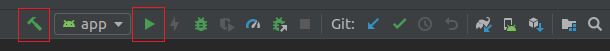
\includegraphics[scale=0.9]{./images/AndroidStudio.PNG}
	\caption{\textit{Tasti Build e Run}}\label{martello}
\end{figure}

\newpage
\section{Installazione skill}
\label{installazioneSkill}
Per ognuno dei sequenti comandi è richiesta l'installazione del package manager \textbf{npm}.
Installazione della skill e delle sue dipendenze:
\begin{itemize}
    \item clonare la repository attraverso il comando \textit{git clone\\https://github.com/sgt390/MegAlexaSkill/};
    \item eseguire il comando \textit{npm install} per installare automaticamente le dipendenze.
\end{itemize}
Pubblicare la skill in AWS Lambda:
\begin{itemize}
    \item installare il programma \textit{7z$_{G}$} e inserire il suo eseguibile tra le variabili di sistema;
    \item installare e configurare aws-cli\footnote{\url{https://aws.amazon.com/it/cli/}};
    \item da terminal, eseguire il comando \textit{npm run publish-lambda}.
\end{itemize}
Eseguire i test di unità:
\begin{itemize}
    \item da terminal, eseguire il comando \textit{npm run unitTest}.
\end{itemize}
Eseguire i test di integrazione:
\begin{itemize}
    \item da terminal, eseguire il comando \textit{npm integrationTest}.
\end{itemize}
